\section{Organisation}

\subsection{Les outils utilisés}

Le projet a été codé en langage C sous systèmes de type Unix. L’affichage graphique a été réalisé à l’aide de la
bibliothèque SDL 2.0 qui est déjà utilisée dans de nombreux jeux. Les sprites sont libres de droits. Étant donné l’ampleur du projet et le
nombre de participants, nous nous sommes convenus d’utiliser le gestionnaire de version git. Un dépôt public a été créé sur Github et est accessible à l'adresse suivante : \url{https://github.com/Neressea/projetC}

\subsection{Le planning initial}

Afin d'achever au mieux les objectifs que nous nous étions fixés, nous avons dressé un planning optimal des tâches à effectuer, en les répartissant par priorité. Voici le gantt des objectifs initiaux.

\begin{figure}[!ht]
    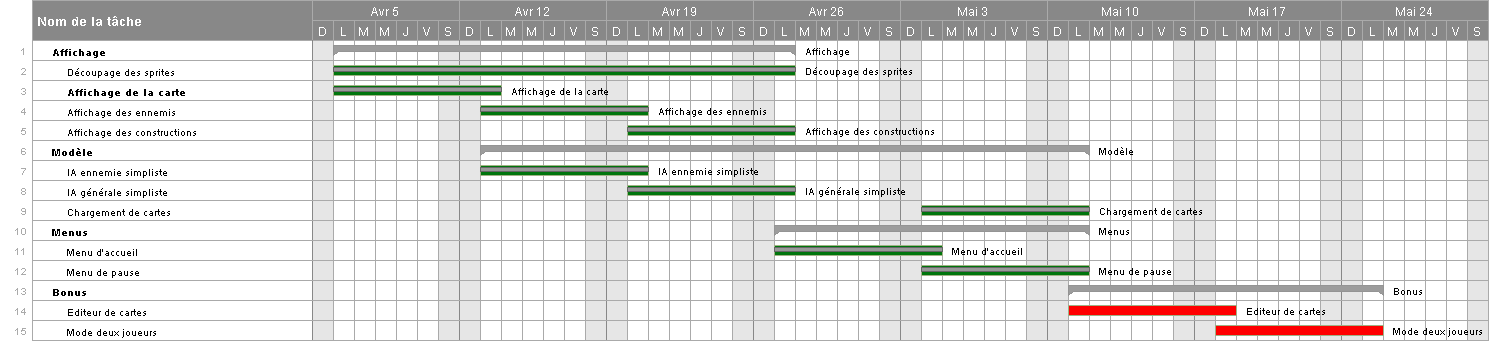
\includegraphics[width=1.1\textwidth]{./images/gantt.png}
    \caption{Gantt du projet}
\end{figure}

Nous n'avons malheureusement pas eu le temps d'ajouter toutes les fonctionnalités optionnelles que nous avions prévu de faire. Cependant, nous en avons aussi ajouté de nouvelles en cours de développement .

\subsection{UML des fichiers et fonctionnalités}

Voici le schéma simplifié de la structure des fichiers. Seuls les structures et fonctions les plus importantes ont été représentées afin de conserver la lisibilité du schéma. 

\begin{figure}[!ht]
    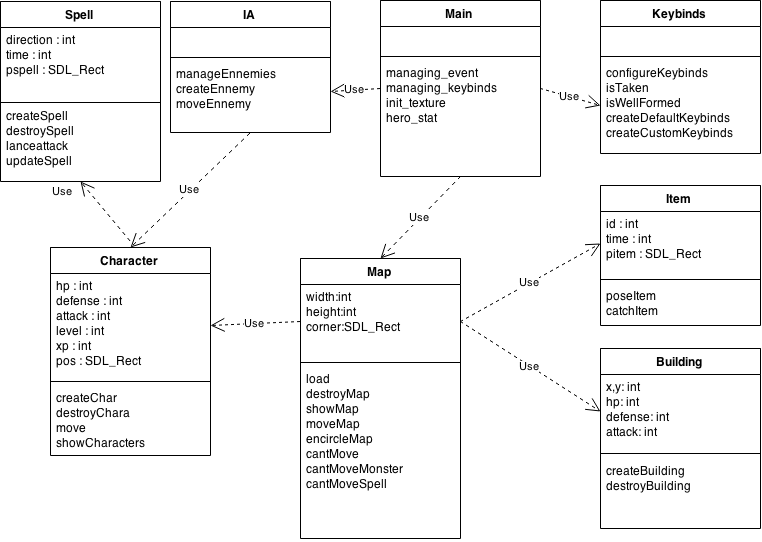
\includegraphics[width=1\textwidth]{./images/uml.png}
    \caption{UML}
\end{figure}

On peut remarquer l'organisation structurelle du code qui tend à se rapprocher d'un code objet. Les listes chaînées n'ont pas été représentées afin de ne pas encombrer l'UML.

